\documentclass{standalone}

\usepackage{tikz}
\usepackage{amsmath,amssymb,amsfonts,amsthm}

\begin{document}

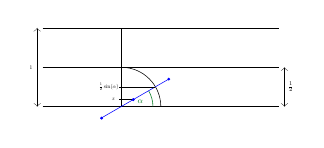
\begin{tikzpicture}

\definecolor{dunkelg}{RGB}{0,119,30};

\draw[very thin] (0,0)   -- (3,0);
\draw[very thin] (0,0.5) -- (3,0.5);
\draw[very thin] (0,1)   -- (3,1);

\draw[very thin] (1,0) -- (1,1);

\draw[<->,ultra thin] (-0.07,0) -- (-0.07,1);
\draw[<->,ultra thin] (3.07,0) -- (3.07,0.5);

\draw[very thin] (1.5,0)  arc[radius = 5mm, start angle= 0, end angle= 90];

\draw[very thin,blue] (1.6,0.35) -- +(210:1cm);

\draw[very thin,dunkelg] (1.4,0)  arc[radius = 4mm, start angle= 0, end angle= 30];

\draw[fill,blue] (0.748,-0.145) circle [radius = 0.01];
\draw[fill,blue] (1.6,0.35) circle [radius = 0.01];
\draw[fill,blue] (1.15,0.09) circle [radius = 0.01];


\draw[ultra thin] (0.97,0.253) -- (1.43,0.253);

\node[scale = 0.3] at (3.15,0.25) {$\frac{1}{2}$};
\node[scale = 0.2] at (-0.15,0.5) {$1$};
\node[scale = 0.2] at (0.9,0.09) {$x$};
\node[scale = 0.2] at (0.84,0.253) {	$\frac{1}{2} \sin(\alpha)$};

\node[scale = 0.3,dunkelg] at (1.24,0.06) {$\alpha$};
\draw[ultra thin] (0.97,0.09) -- (1.15,0.09);

\draw[fill,blue] (1.15,0.09) circle [radius = 0.01];
\end{tikzpicture}


\end{document}